% $Id: calculations-quark-gluon.tex 529 2019-12-12 10:54:11Z smarzani $
%
% This contains calculations for quark-gluon discrimination
%------------------------------------------------------------------------

%%========================================================================
\chapter{Quark/gluon discrimination}\label{sec:calc-shapes-qg}

\begin{figure}
  \centerline{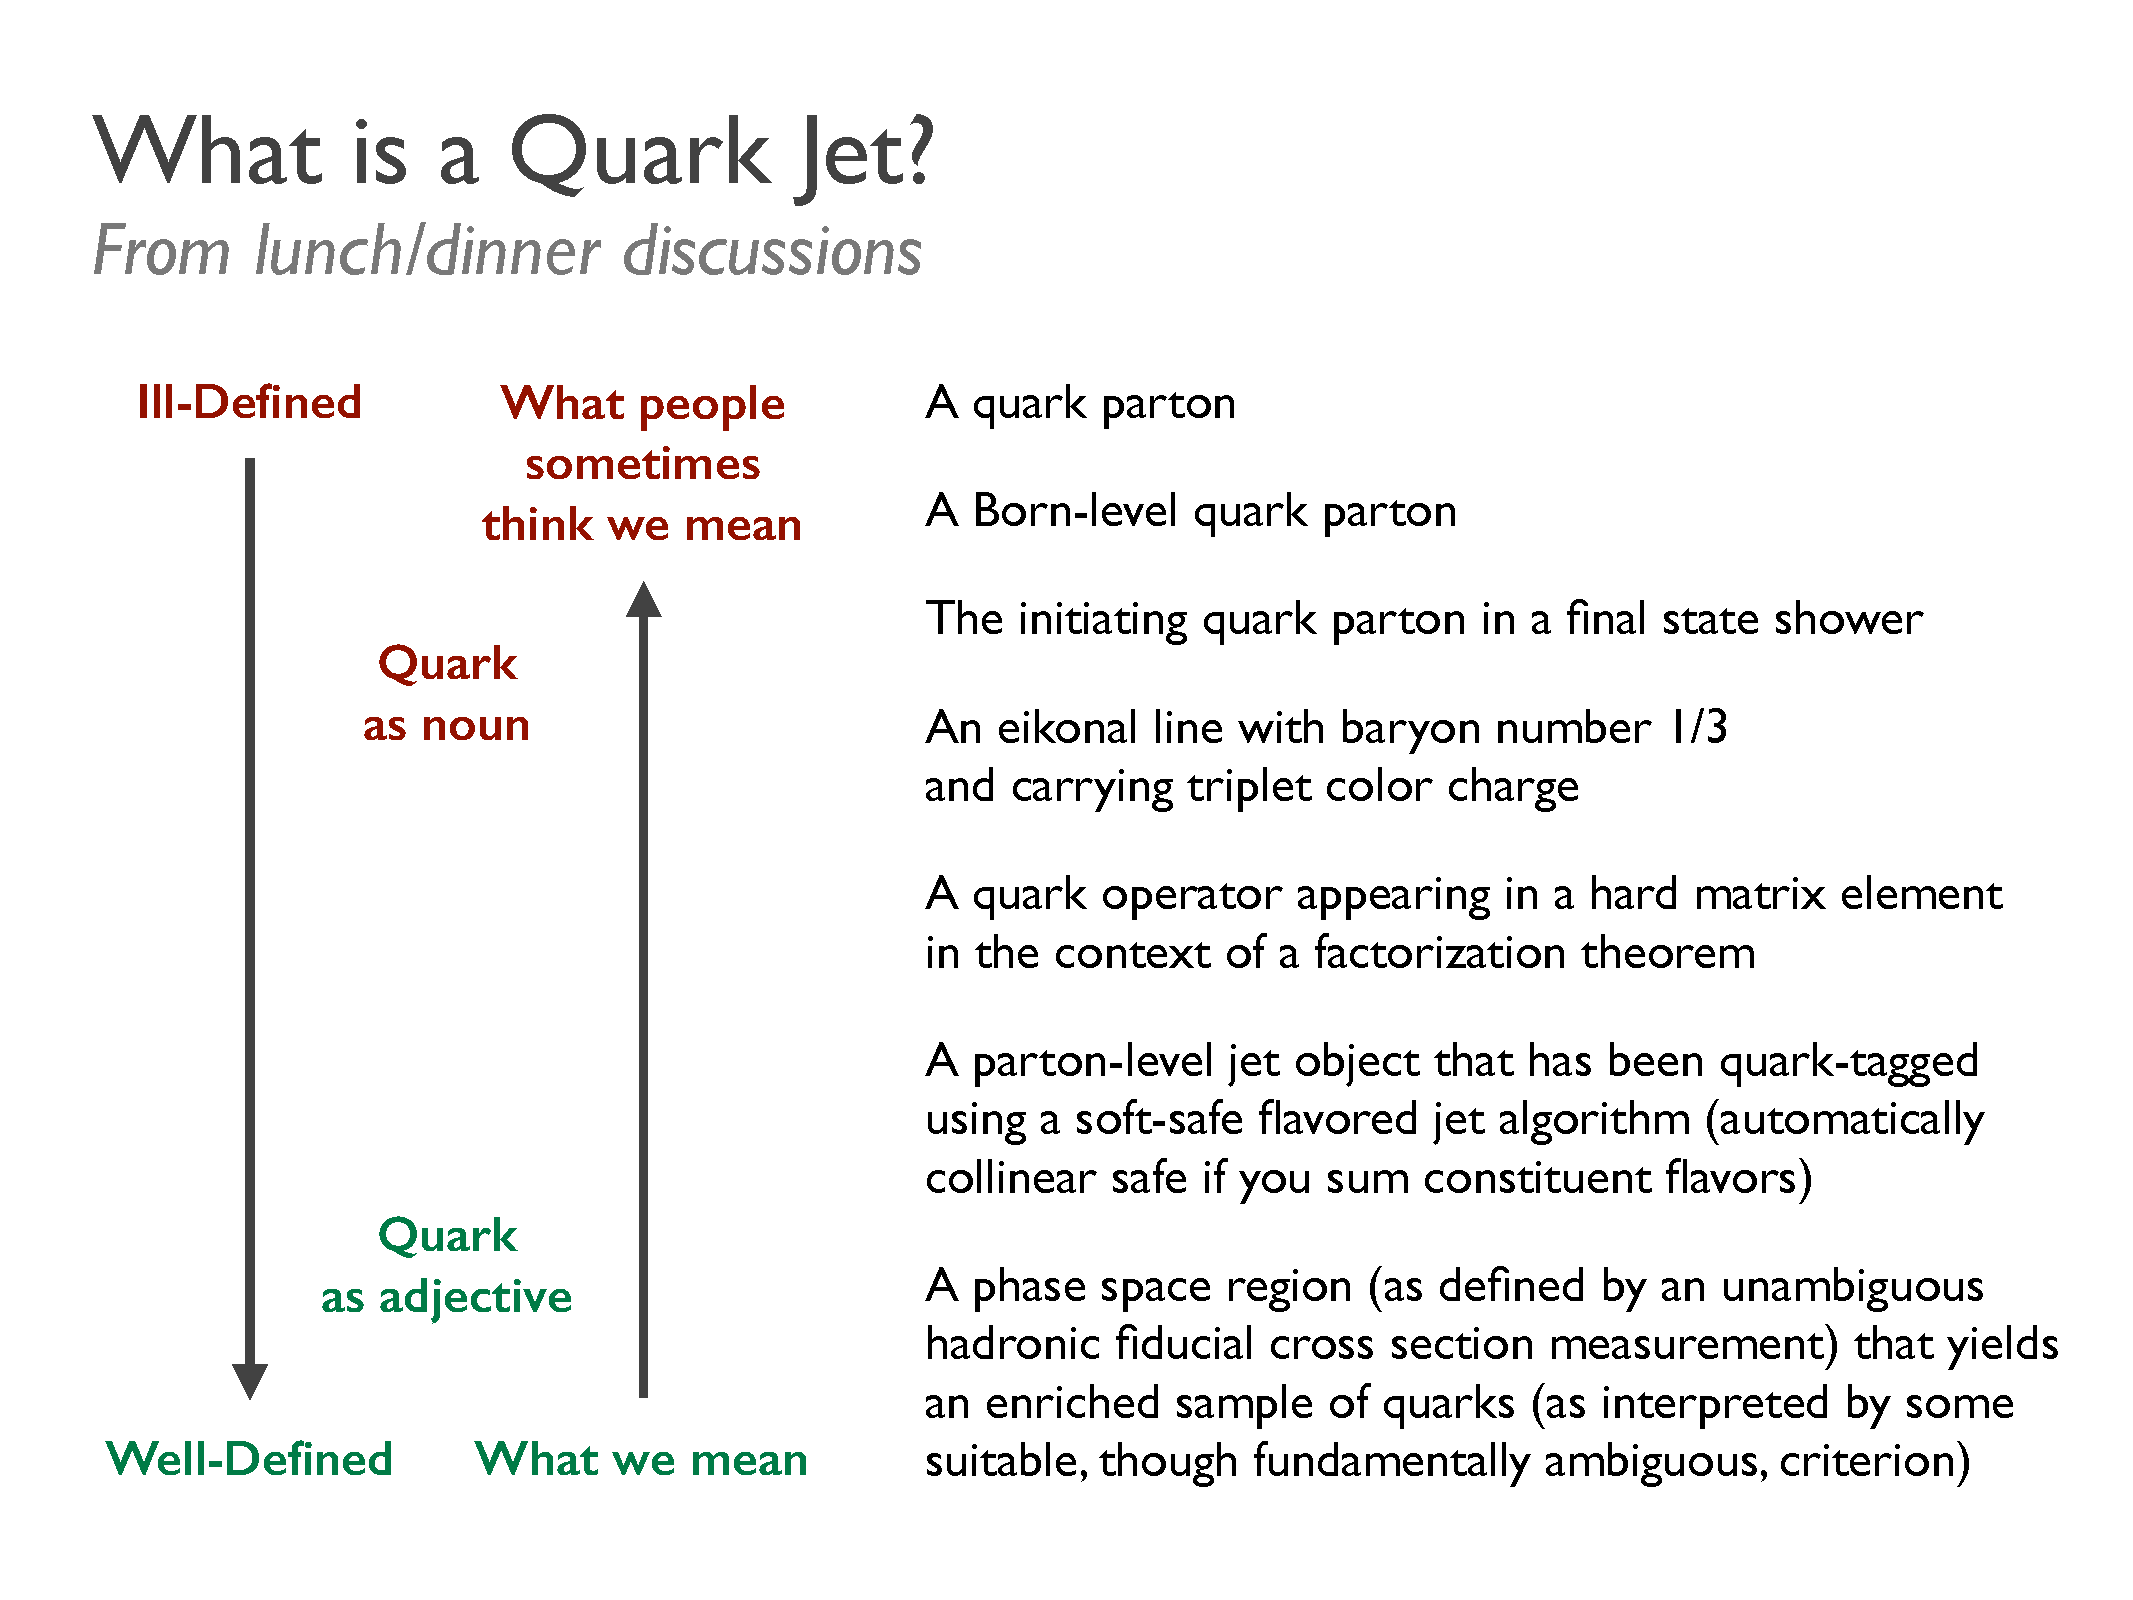
\includegraphics[width=0.75\textwidth]{figures/quark-gluon-jet-definitions.pdf}}
  \caption{Possible definitions of a ``quark jet'' or a
    ``gluon jet'' (from Ref.~\cite{Badger:2016bpw}, see also~\cite{Gras:2017jty}).}\label{fig:qgjet-defs}
\end{figure}

In this chapter we discuss the application of jet substructure tools
for discriminating between quark- and gluon-initiated jets.
%
Before digging into the substructure aspects of the matter, let us
briefly mention that there are many ways to define what a ``quark
jet'' or a ``gluon jet'' is. Several possibilities are listed in
Fig.~\ref{fig:qgjet-defs}. Amongst these possible definitions, many
are clearly pathological, simply because a parton is not a physically
well-defined object (cf. also our discussion about jets in
Chapter~\ref{chap:jets-and-algs}).
%
What is well-defined is a measurable quantity, that one can associate
(in an inevitably ambiguous way) to an enriched sample of quarks or
gluons.
%
For simplicity, we often rely on event samples involving hard quarks
or gluon in the Born-level process, but one has to be aware that this
is not unambiguously defined approach and keep this in mind when interpreting
the results.
%
This is what we have already done in the previous chapter when
generating $qq\to qq$ Pythia8 events as a proxy for quark jets and
this is again what we will do here.
%
Note that the better-defined definition in Fig.~\ref{fig:qgjet-defs}
depends on which sample is used. An investigation of this dependence
can be found in~\cite{Bright-Thonney:2018mxq}.

That said, several processes one wants to measure at the LHC, like
Higgs production through vector-boson-fusion, or new-physics events, such as cascades of supersymmetric particles, tend to
produce quark jets while QCD backgrounds are gluon-dominated. This
motivates the use of substructure tools to try and discriminate between
the two.
%
Some years ago, a wide range of discriminants
has been systematically studied and
compared~\cite{Gallicchio:2012ez}.
%
It is not our goal to go through all the details of this
study. Instead, we have selected a few representative discriminators
and discussed their performance and their basic analytic properties.
%
We focus on two main categories of tools: jet shapes, namely
angularities and energy-correlation functions, and multiplicity-based
observables, namely the iterated \SD multiplicity.
%
We conclude this chapter with a comparison of their performance (in
the sense of Sec.~\ref{sec:performance-intro}) using Monte Carlo
simulations.

Our Monte Carlo studies use Pythia8 (with the Monash13 tune). We
generate ``quark-initiate jets'' using $qg\to \text{Z}q$ hard matrix
elements and ``gluon-initiated jets'' using $q\bar q\to \text{Z}g$
events. In both cases, the Z boson is made to decay into invisible
neutrinos and we focus on the hardest anti-$k_t$($R=0.5$) jet in the
event requiring $p_t>500$~GeV.

\section{Angularities, ECFs and Casimir scaling}

The motivation behind using jet shapes for quark-gluon discrimination
is the observation that gluons tend to radiate more than quarks and jet shapes are
precisely a measure of this radiation.
%
Typical examples of shapes that can be used in this context are the
angularities $\lambda_\alpha$ and the energy-correlation functions (ECFs)
$e_2^{(\alpha)}$, introduced in
Sec.~\ref{sec:tools-radiation-constraints}.
%
In both cases, one would expect a larger value of
$v=\lambda_\alpha,e_2^{(\alpha)}$ for gluon jets than for quark jets
and one can build an enhanced quark sample by simply imposing a cut
$v<v_\text{cut}$.

We will first perform some analytic calculations for angularities and ECFs,
before discussing their performance as quark-gluon separators. We will
come back to this in Sec.~\ref{sec:qg-perf-robustness}, where we
also discuss their robustness against non-perturbative effects.

\paragraph{Analytic behaviour.}
%
For the purpose of the physics discussion we want to have, we will
need a resummed calculation at NLL accuracy.
%
At this accuracy, angularities and ECFs have the same structure,
provided one uses a recoil-insensitive jet axis definition
for angularities with $\alpha\le 1$.
%
This is easy to explain from a simple one-gluon emission argument (cf.\ \eg
Fig.~\ref{fig:mmdt-mass-one-gluon}). If $\theta$ denotes the angle
between the emitted soft gluon and the recoiling hard parton, a
standard four-vector recombination scheme, e.g.\ the E-scheme, would give an angle
$(1-z)\theta$ between the soft gluon and the jet axis and an angle
$z\theta$ between the recoiling hard parton and the jet axis.  This
gives
%
\begin{equation}
\lambda_\alpha^\text{(E-scheme)}=z[(1-z)\theta]^\alpha + (1-z)[z\theta]^\alpha=[z(1-z)^\alpha+(1-z)z^\alpha]\theta^\alpha,
\end{equation}
where the first contribution comes from the soft gluon and the second
from the recoiling parton.
%
For $\alpha=1$, both partons contribute equally to give
$\lambda_1^\text{(E-scheme)}=2z(1-z)\theta\approx 2z\theta$. This
leaves the LL behaviour unaffected but introduces recoil effects at
NLL (with a resummation structure more complex than the simple
exponentiation in~(\ref{eq:Sigma-plain-jet-mass}).
%
For $\alpha<1$, $\lambda_\alpha^\text{(E-scheme)}
\approx z^\alpha\theta^\alpha$ dominated by the recoil of the hard
parton, so recoil effects are already present at LL.
%
If we use the winner-takes-all (WTA) axis --- what we did in
practice in our Monte Carlo simulations --- angularities become
recoil-free and we have
\begin{equation}
  \lambda_\alpha^\text{(WTA)}=z\theta^\alpha.
\end{equation}
%
This effect is not present for ECFs for which we have
$e_2^\alpha = z(1-z)\theta^\alpha\overset{z\ll
  1}{\approx}z\theta^\alpha$, independently of the recombination
scheme.

For $\alpha=2$, angularities and ECFs are essentially equivalent to
the mass --- more precisely $m^2/(p_tR)^2$ --- and we can reuse the
same results as in Chapter~\ref{chap:calculations-jets}. 
%
These results can almost trivially be extended to a generic value of
the angular exponent $\alpha$. First, we need expressions for the
radiators valid at NLL. This requires including the two-loop
running-coupling corrections in the CMW scheme (see the discussion
before Eq.~\eqref{eq:radiator-nll-expansion}).
%
For the plain jet, one finds a generalisation of Eqs.~(\ref{eq:quark})
and~\eqref{eq:radiator-nll-contribution}:
\begin{align}\label{eq:plain-angularity-radiator-nll}
  R_\text{plain}^{\text{(NLL)}}(v)
   = \frac{C_i}{2\pi\alpha_s\beta_0^2}&\Bigg\{
    \bigg[\frac{1}{\alpha-1}W(1-\lambda)-\frac{\alpha}{\alpha-1}W(1-\lambda_1)+W(1-\lambda_B)\bigg]\\
  & +\frac{\alpha_s\beta_1}{\beta_0}\bigg[
\frac{1}{\alpha-1}V(1-\lambda)-\frac{\alpha}{\alpha-1}V(1-\lambda_1)+V(1-\lambda_B)
    \bigg]\nonumber\\
    & -\frac{\alpha_sK}{2\pi}\bigg[
\frac{1}{\alpha-1}\log(1-\lambda)-\frac{\alpha}{\alpha-1}\log(1-\lambda_1)+\log(1-\lambda_B)
    \bigg]\Bigg\},\nonumber
\end{align}
where $W(x)=x\log(x)$, $V(x)=\tfrac{1}{2}\log^2(x)+\log(x)$ and we have introduced 
\begin{equation}
  \lambda = 2\alpha_s\beta_0\log(1/v),\qquad
  \lambda_B = -2\alpha_s\beta_0 B_i,\qquad\text{and}\quad
  \lambda_1  = \frac{\lambda+(\alpha-1)\lambda_B}{\alpha}.
\end{equation}
Before discussing these results, let us point out that one can also
apply grooming to the jet, using mMDT or \SD, and compute the shape on
the groomed jet. In this case, we get the same as 
Eq.~(\ref{eq:plain-angularity-radiator-nll}) for $v>\zcut$ and a generalisation of
Eq.~(\ref{eq:mMDTSD-radiator-modll}) for $v< \zcut$:
\begin{align}\label{eq:sd-angularity-radiator-nll}
  \MoveEqLeft[1] R_\text{mMDT/SD}^{\text{(NLL)}}(v) = \\
  & = \frac{C_i}{2\pi\alpha_s\beta_0^2}\Bigg\{
    \bigg[\frac{(\alpha+\beta)W(1-\lambda_2)}{(\beta+1)(\alpha-1)}-\frac{\alpha
    W(1-\lambda_1)}{\alpha-1}-\frac{W(1-\lambda_c)}{\beta+1}+W(1-\lambda_B)\bigg]\nonumber\\
  & \phantom{=\frac{C_i}{2\pi\alpha_s\beta_0^2}}
    +\frac{\alpha_s\beta_1}{\beta_0}\bigg[
\frac{(\alpha+\beta)V(1-\lambda_2)}{(\beta+1)(\alpha-1)}-\frac{\alpha
    V(1-\lambda_1)}{\alpha-1}-\frac{V(1-\lambda_c)}{\beta+1}+V(1-\lambda_B)    \bigg]\nonumber\\
  & \phantom{=\frac{C_i}{2\pi\alpha_s\beta_0^2}}
    -\frac{\alpha_sK}{2\pi}\bigg[
\frac{(\alpha+\beta)\log(1-\lambda_2)}{(\beta+1)(\alpha-1)}-\frac{\alpha
    \log(1-\lambda_1)}{\alpha-1}-\frac{\log(1-\lambda_c)}{\beta+1}+\log(1-\lambda_B) \bigg]\Bigg\},\nonumber
\end{align}
with 
\begin{equation}
 \lambda_c = 2\alpha_s\beta_0\log(1/\zcut),
 \qquad\text{and}\quad
 \lambda_2 = \frac{(\beta+1)\lambda+(\alpha-1)\lambda_c}{\alpha+\beta}.
\end{equation}

These expressions require a few comments. First of all,
Eq.~(\ref{eq:plain-angularity-radiator-nll}), for $\alpha=2$, slightly
differs from Eqs.~(\ref{eq:quark})
and~\eqref{eq:radiator-nll-contribution}.
%
The difference is in the treatment of the $B$ term which corresponds
to hard collinear splittings where, as in
Chapter~\ref{calculations-substructure-mass}
(cf.~(\ref{eq:mMDTSD-radiator-modll-altB})), we have inserted the
contribution from hard-collinear splittings in the double-logarithmic
terms (see also Appendix~\ref{chap:app-analytic-details} for a
discussion on how to do this in practice).
%
One can also notice that the limit $\beta\to\infty$
of~Eq.~(\ref{eq:sd-angularity-radiator-nll}) gives back
Eq.~(\ref{eq:plain-angularity-radiator-nll}) as expected.
%
Furthermore, taking $\alpha=2$ in the mMDT/\SD case and neglecting the
two-loop corrections, one recovers
Eq.~(\ref{eq:mMDTSD-radiator-modll-altB}).
%
Finally, we note that, although the above results have factors of $\alpha-1$ in the
denominator, they are finite for $\alpha\to 1$ (corresponding to the
specific case of broadening or girth for angularities). 

Given the above radiators, we can compute the probability that the
angularity (or ECF) has a value smaller than $v$, i.e.\ the cumulative distribution, at NLL:
\begin{equation}\label{eq:angularities-nll-cumul}
  \Sigma^\text{(NLL)}(v) = \frac{e^{-R(v)-\gamma_E R'(v)}}{\Gamma(1+R'(v))},
\end{equation}
where the factor $e^{-\gamma_E R'(v)}/[\Gamma(1+R'(v))]$ accounts for
multiple emissions (cf.~(\ref{eq:mult-emission-nll})), and $R'(v)$ is
the derivative of $R(v)$ with respect to $\log(1/v)$. Since the multiple-emission
correction is already subleading, $R'$
in~\eqref{eq:angularities-nll-cumul} can be computed from the LL terms
in $R$ and we get (again, keeping the $B$ term only to guarantee an
endpoint at $\log(v)=B_i$)\footnote{In practice, this definition of
  $R'_\text{mMDT/SD}(v)$ introduces a discontinuity in the
  differential distribution at $v=\zcut$. This discontinuity is
  strictly-speaking subleading and can be avoided by defining $R'$
  using a finite-difference derivative:
  $R'(v)=[R(v e^{-\Delta})-R(v)]/\Delta$, with $\Delta$ a constant
  number, which respects NLL accuracy
  (see~\cite{Larkoski:2014wba}). This is what we have done for the
  results presented below, using $\Delta=0.5$.}
\begin{align}\label{eq:angularities-Rp}
R'_\text{plain}(v) & = \frac{C_i}{\pi\beta_0}\frac{1}{\alpha-1}\log\bigg(\frac{1-\lambda_1}{1-\lambda}\bigg),\\
R'_\text{mMDT/SD}(v) & = \frac{C_i}{\pi\beta_0}\frac{1}{\alpha-1}\log\bigg(\frac{1-\lambda_1}{1-\lambda_2}\bigg).
\end{align}
Note finally that while Eq.~\eqref{eq:angularities-nll-cumul} is only
correct in the small jet radius limit and should include soft
wide-angle emissions and non-global logs to reach full NLL accuracy,
Eq.~\eqref{eq:angularities-nll-cumul} includes all the NLL
contributions for Soft-Dropped angularities which are insensitive to soft
wide-angle emissions.

\begin{figure}
  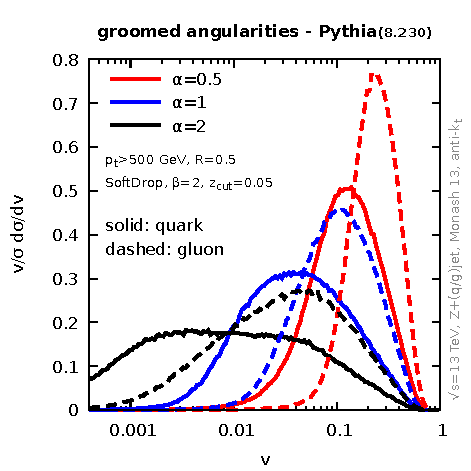
\includegraphics[width=0.48\textwidth,page=1]{figures/groomed-angularities-pythia.pdf}%
  \hfill%
  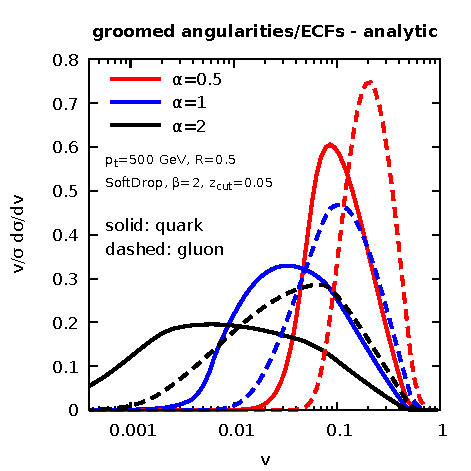
\includegraphics[width=0.48\textwidth,page=1]{figures/groomed-angularities-analytic.pdf}%
  \caption{Distribution of a sample of groomed angularities for quark
    (solid lines) and gluon (dashed lines) jets. The left plot
    corresponds to parton-level Pythia simulations and the right plot
    to the analytic results obtained in these lecture
    notes.}\label{fig:grm-ang-v-alpha}
\end{figure}  

\begin{figure}
  \includegraphics[width=0.48\textwidth,page=2]{figures/groomed-angularities-pythia.pdf}%
  \hfill%
  \includegraphics[width=0.48\textwidth,page=2]{figures/groomed-angularities-analytic.pdf}%
  \caption{Same as Fig.~\ref{fig:grm-ang-v-alpha}, this time for a
    fixed angularity $\lambda_1$, varying the
    groomer.}\label{fig:grm-ang-v-beta}
\end{figure}  

\paragraph{Comparison to Monte Carlo.}
%
A comparison between the above
analytic predictions and parton-level Monte Carlo simulations are
shown in Fig.~\ref{fig:grm-ang-v-alpha}, for different values of the angularity
exponent for \SD jets, and in Fig.~\ref{fig:grm-ang-v-beta}, for different
levels of grooming for $\lambda_{\alpha=1}$.
%
Overall, we see that there is a good agreement between the analytic
calculation and the Monte Carlo simulations.
%
We recall that our resummed calculation should not be trusted in the
region of large $v$ where an exact fixed-order calculation would be
needed. This could be obtained from NLO Monte Carlo generators like
NLOJet++~\cite{Nagy:2003tz} for dijet hard processes (here one would
need a 3-jet NLO calculation for the angularity distribution) and
MCFM~\cite{Campbell:1999ah,Campbell:2011bn,Campbell:2015qma} for
W/Z+jet events (here we would need W/Z+2 jets at NLO for the
angularity distribution).
%
The NLO distributions could then be matched to the resummed calculation
to obtain a final prediction which is valid at the same time in the
resummation-dominated region (small angularity) and in the
fixed-order-dominated region (large angularity).
%
More importantly, Figs.~\ref{fig:grm-ang-v-alpha}
and~\ref{fig:grm-ang-v-beta} show the expected clear separation
between the quark and gluon samples, with smaller values of the
angularity for the quark jets.


\begin{figure}
  \centering
  \subfloat[]{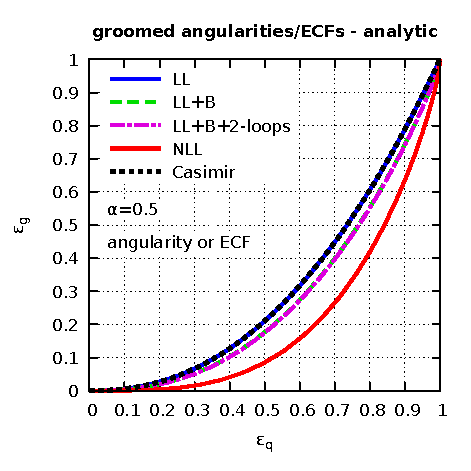
\includegraphics[width=0.48\textwidth,page=1]{figures/groomed-angularities-roc-casimir.pdf}\label{fig:grm-ang-casimir}}%
  \hfill%
  \subfloat[]{\includegraphics[width=0.48\textwidth,page=3]{figures/groomed-angularities-roc-pythia.pdf}\label{fig:grm-ang-ptdep}}%
  \caption{Left: analytic predictions for the quark-gluon separation
    ROC curve using different approximations. Right: ROC curve for
    different values of $p_t$, shown for both Pythia8 simulations
    (solid) and our analytic calculation (dashed).}\label{fig:grm-ang-basicprops}
\end{figure}  


\paragraph{Quark-gluon discrimination and Casimir scaling.}
%
With the above results at hand, we can finally discuss the performance
of angularities and energy-correlation functions to separate quark
jets from gluon jets. This is simply done by imposing a cut
$v<v_\text{cut}$ on angularities or ECFs.
%
On the analytic side, the quark and gluon efficiencies are therefore
directly given by $\Sigma_{q,g}$  computed above.
%
An interesting behaviour emerges from these analytic results. If we
look at Eqs.~(\ref{eq:plain-angularity-radiator-nll})
and~(\ref{eq:sd-angularity-radiator-nll}) at leading-logarithmic
accuracy, the only difference between quark and gluon jets is the
colour factor --- $C_F$ for quarks and $C_A$ for gluons, in from of
the radiators. This means that we have
\begin{equation}\label{eq:casimir-scaling}
\epsilon_g \overset{\text{LL}}{=} (\epsilon_q)^{C_A/C_F}.
\end{equation}
%
This relation is often referred to as {\em Casimir scaling}~(see
\eg~\cite{Larkoski:2013eya}). This means that the leading behaviour of
quark-gluon tagging will follow Eq.~(\ref{eq:casimir-scaling}) regardless
of the angularity (of ECF) exponent and of the level of grooming.

Departures from Casimir scaling will start at NLL accuracy. In our
collinear/small-$R$ limit, these means that there can be three sources of
Casimir-scaling violations: hard-collinear corrections (the $B$ term),
two-loop running-coupling corrections, and multiple-emissions
(cf. Eq.~(\ref{eq:angularities-nll-cumul})). 
%
Of these three effects, only the first and the last give scaling
violations since two-loop running coupling corrections are also simply
proportional to $C_i$.
%
This is illustrated in Fig.~\ref{fig:grm-ang-casimir}, where we see
that the LL result gives perfect Casimir scaling, and the inclusion of
the hard collinear splitting and the multiple-emission corrections
both slightly increase the quark-gluon discrimination performance.
%
The correction due to the $B$-term is proportional to $B_g-B_q$ which
is small and positive. The effect of multiple emissions starts at
${\cal {O}}(\alpha_s^2)$ in the perturbative expansion and is
proportional to $(C_A-C_F)$.
%
In practice, this last effect appears to have the largest impact.
%
A direct consequence of Casimir scaling is that the quark-gluon
discriminative power remains relatively independent of the jet $p_t$
as shown on Fig.~\ref{fig:grm-ang-ptdep} for both our analytic
calculation (dashed lines) and Pythia8 parton-level simulations (solid
lines).

\begin{figure}
  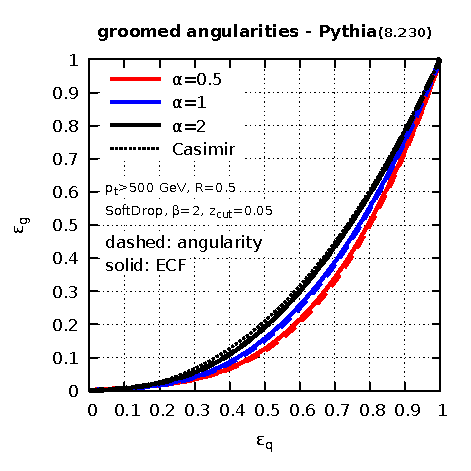
\includegraphics[width=0.48\textwidth,page=1]{figures/groomed-angularities-roc-pythia.pdf}%
  \hfill%
  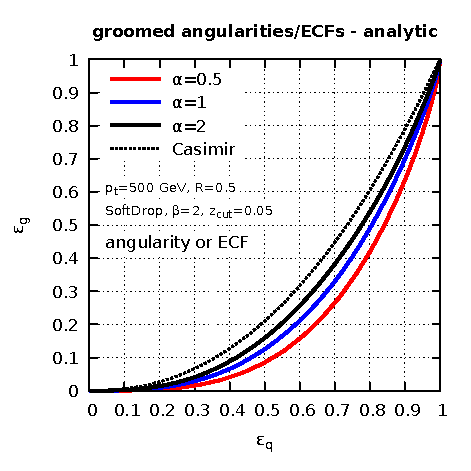
\includegraphics[width=0.48\textwidth,page=1]{figures/groomed-angularities-roc-analytic.pdf}%
  \caption{ROC curves for quark/gluon separation using ECFs (solid lines) and angularities (dashed lines). The left plot
    corresponds to parton-level Pythia simulations and the right plot
    to the analytic results obtained in these lecture
    notes.}\label{fig:grm-ang-roc-v-alpha}
\end{figure}  


All these effects are discussed at length in
Ref.~\cite{Larkoski:2013eya} and we refer the reader to this
discussion for further details.
%
ROC curves for quark-gluon discrimination
are shown in Fig.~\ref{fig:grm-ang-roc-v-alpha} for both Pythia (at
parton level) and our analytic calculation, for jets groomed with \SD.
%
We see a good level of agreement between the two although the
analytic results tend to produce a slightly larger quark-gluon
discrimination that Pythia.
%
It is however notorious that different Monte Carlo generators tend to predict
relatively different deviations from Casimir scaling, both at parton and hadron level. We refer to Ref.~\cite{Gras:2017jty} for more
details about this. 
%
Above all, we conclude from Fig.~\ref{fig:grm-ang-roc-v-alpha} that smaller
values of $\alpha$ give better discrimination, with very similar
results obtained for angularities and energy-correlation functions.
%
We will come back to this in Sec.~\ref{sec:2prongs-perf-robustness}
when discussing the performance and robustness of quark-gluon
discriminators.


\section{Beyond Casimir scaling with Iterated SoftDrop}\label{sec:isd}

Given the observation made in the previous section that angularities
and energy-cor\-relation functions produce quark-gluon discriminators
which depart from Casimir scaling only due to subleading corrections,
it is natural to wonder if it is possible to find substructure tools
which have a different behaviour already at leading-logarithmic
accuracy.

The behaviour one would want to obtain is a Poisson-like
behaviour like what the particle multiplicity in a jet, or the
charged-track multiplicity, typically achieve.
%
In this section, we discuss a tool, namely the {\em Iterated SoftDrop (ISD)
  multiplicity} introduced in Sec.~\ref{sec:def-other-shapes} and
show that it achieves a Poisson-like behaviour already at LL while
remaining infrared-and-collinear safe (contrary to particle or
charged-track multiplicity).
%
As above, we will first briefly discuss the analytic structure of ISD
multiplicity and compare the resulting performance with Monte-Carlo
simulations.

\paragraph{ISD Multiplicity at LL.}
%
The main interesting features of ISD multiplicity already arise at
leading logarithmic accuracy, so we will focus on this in what
follows.
%
The key observation is that at LL, all the emissions from the hard
(leading) parton are soft and collinear, strongly ordered in angle and
independent from one another. The fact that the emissions are
independent automatically guarantees that, if $\nu$ is the probability
that one emission is counted by the ISD de-clustering procedure, \ie
passes the \SD condition, then the probability to have $n$ emission
passing the \SD condition follows a Poisson distribution
\begin{equation}\label{eq:isd-poisson}
\frac{1}{\sigma} \frac{d\sigma}{dn_\text{ISD}} = e^{-\nu} \frac{\nu^n_\text{ISD}}{n_\text{ISD}!}.
\end{equation}

We now need to compute $\nu$ explicitly.
%
This is straightforward since, at LL, the probability to have an emission that passes the \SD condition is simply
given by (measuring angles in units of the jet radius as usual)
\begin{equation}
\nu = \int_0^1
\frac{d\theta^2}{\theta^2}dz\,P_i(z)\frac{\alpha_s(z\theta p_tR)}{2\pi} \Theta(z>\zcut\theta^\beta).
\end{equation}
For the ISD multiplicity to be IRC-safe, $\nu$ has to remain
finite. This can easily be achieved by using a negative value for
$\beta$, guaranteeing a finite phase-space for the emissions (cf. \eg
the Lund diagram of Fig.~\ref{fig:lund-sd}).
%
Alternatively, we can manually impose a minimum $k_t$ cut,
$z\theta>\kappa_\text{cut}$, on the emissions which pass the \SD
condition, or stop the iterative de-clustering procedure at a minimum
angle $\theta_\text{cut}$.

\begin{figure}
    \centering
    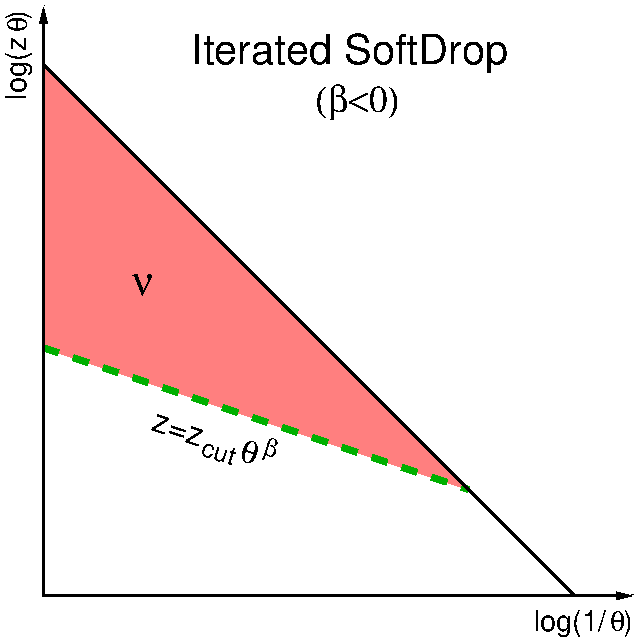
\includegraphics[width=0.32\textwidth]{figures/Lund-ISD-negb.pdf}%
    \hfill%
    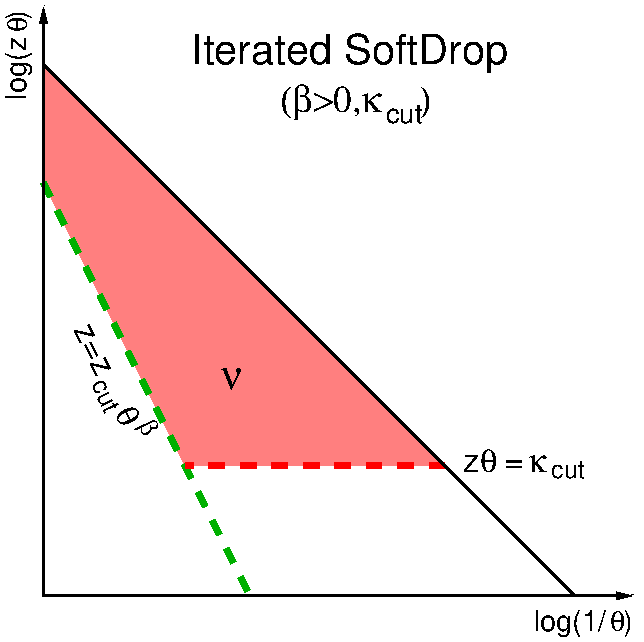
\includegraphics[width=0.32\textwidth]{figures/Lund-ISD-posb-ktcut.pdf}%
    \hfill%
    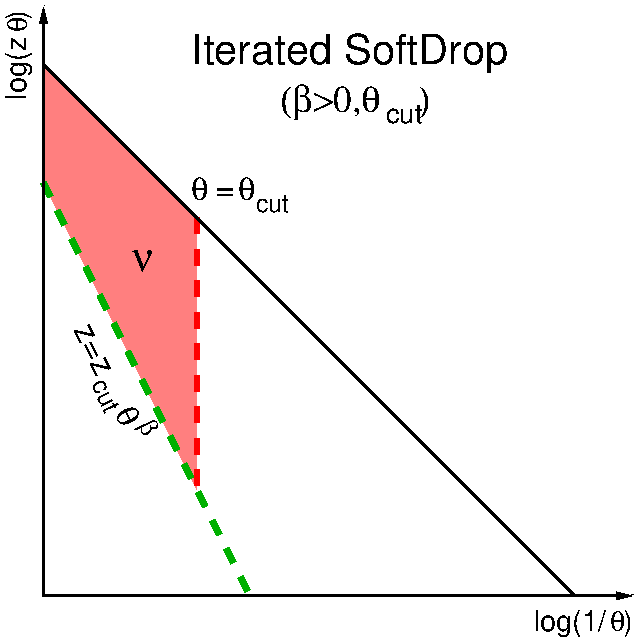
\includegraphics[width=0.32\textwidth]{figures/Lund-ISD-posb-thetacut.pdf}
    \caption{Lund diagrams representing the regions in which Iterated
      \SD counts the emissions. From left to right we have $\beta<0$,
      $\beta>0$ with a cut on $k_t$ and $\beta>0$ with an angular cut.
    }\label{fig:lund-isd-lund}
\end{figure}

These three options correspond to the three regions of the Lund
diagram shown in Fig.~\ref{fig:lund-isd-lund}.
%
The corresponding analytic expressions for $\nu$ can be obtained
exactly as for the radiators computed for angularities in the previous
Section (this time keeping only LL term, and hard collinear
splittings). One finds (assuming $\kappa<\zcut$ for the second
case):\footnote{These first two results can be directly derived
  from Eq.~(\ref{eq:plain-angularity-radiator-nll})
  and Eq.~(\ref{eq:sd-angularity-radiator-nll}). The third corresponds to
  the radiator for the \SD grooming radius originally computed in
  Ref.~\cite{Larkoski:2014wba} and discussed in Sec.~\ref{sec:thetag}
  below.}
\begin{align}
  \nu_{\beta<0} & 
   = \frac{C_i}{2\pi\alpha_s\beta_0^2}
    \bigg[\frac{-1}{1+\beta}W(1-\lambda_c)-\frac{\beta}{1+\beta}W\Big(1+\frac{\lambda_c}{\beta}\Big)\bigg]-\frac{C_i}{\pi\beta_0}
                   \log\Big(1+\frac{\lambda_c}{\beta}\Big)B_i,\label{eq:isd-nu-betaneg}\\
  \nu_{\beta>0,\kappa} & 
   = \frac{C_i}{2\pi\alpha_s\beta_0^2(1+\beta)}
                         \bigg[-W(1-\lambda_c)-(\lambda_c+\beta)\log(1-\lambda_\kappa)-\lambda_c-\beta\lambda_\kappa\bigg]\nonumber\\
  & -\frac{C_i}{\pi\beta_0} \log(1-\lambda_\kappa)B_i,\\
  \nu_{\beta>0,\theta} & 
   = \frac{C_i}{2\pi\alpha_s\beta_0^2(1+\beta)}
    \bigg[-W(1-\lambda_\theta)-\frac{W(1-\lambda_c)}{1+\beta}+\frac{W(1-\lambda_c-(1+\beta)\lambda_\theta)}{1+\beta}
     \bigg]\nonumber\\
  & -\frac{C_i}{\pi\beta_0} \log(1-\lambda_\theta)B_i,
\end{align}
with
\[
  \lambda_c = 2\alpha_s\beta_0\log\Big(\frac{1}{\zcut}\Big),\quad
  \lambda_\kappa = 2\alpha_s\beta_0\log\Big(\frac{1}{\kappa_\text{cut}}\Big),\quad\text{and}\quad
  \lambda_\theta =
  2\alpha_s\beta_0\log\Big(\frac{1}{\theta_\text{cut}}\Big),
\]
Counting logarithms of $\zcut$, $\kappa_\text{cut}$ and
$\theta_\text{cut}$, all the above expressions show a
double-logarithmic behaviour. An easy way to see this is to compute
$\nu$ using a fixed-coupling approximation (equivalent to taking the
limit $\beta_0\to 0$ in the above results). For example, for the
representative $\beta<0$ case we will use in what follows, one has
\begin{equation}
  \nu_{\beta<0} \overset{\text{f.c.}}{=}
   \frac{\alpha_sC_i}{\pi}\frac{-1}{\beta}\bigg[
   \log^2\Big(\frac{1}{\zcut}\Big)+2B_i\log\Big(\frac{1}{\zcut}\Big)\bigg].
\end{equation}


\begin{figure}
  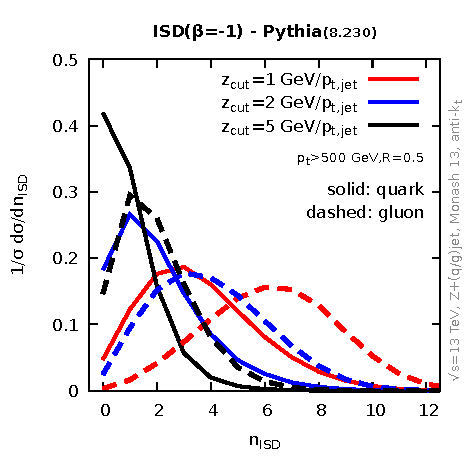
\includegraphics[width=0.48\textwidth]{figures/isd-distribs-pythia.pdf}%
  \hfill%
  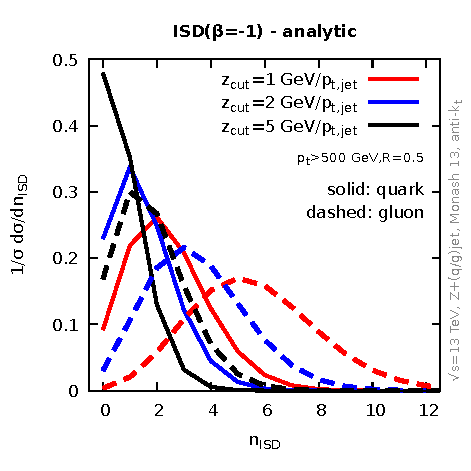
\includegraphics[width=0.48\textwidth]{figures/isd-distribs-analytic.pdf}%
  \caption{Distribution of ISD multiplicity for $\beta=-1$, varying
    $\zcut$. The value of $\zcut$ is given as a dimensionful $k_t$
    scale, normalised to $p_tR$. The left plot
    corresponds to parton-level Pythia simulations (for which $\zcut$
    is re-calculated for each jet) and the right plot
    to the analytic calculation, Eqs.~(\ref{eq:isd-poisson})
    and~(\ref{eq:isd-nu-betaneg}). Solid lines correspond to quark
    jets, while dashed lines correspond to gluon jets.}\label{fig:isd-distrib-v-ktcut}
\end{figure}  

Fig.~\ref{fig:isd-distrib-v-ktcut} shows the ISD multiplicity
distributions for quark and gluon jets, obtained from (parton-level)
Pythia8 simulations (left) and using the analytic expressions above
(right). Each plot shows different values of $\zcut$.
%
For these plots, we have used $\beta=-1$, corresponding to a cut on
the relative $k_t$ of the emissions.
%
To make this more concrete, the value of $\zcut$ is given as a
function of the corresponding $k_t$ cut. In the case of the Pythia8
simulations, the cut has been adapted using the $p_t$ of each
individual jets.
% 
Overall, we see that the analytic calculation captures the main
features of the Monte Carlo simulation, albeit with distributions
which tend to be peaked towards lower multiplicities than in Pythia8.
%
We note that NLL corrections, computed in the initial ISD study,
Ref.~\cite{Frye:2017yrw}, improves the agreement between the
two.
%
One particular effect that becomes relevant at NLL is that the flavour
of the leading branch followed through the ISD declustering can
change. This is included in Pythia8 via the DGLAP splitting functions
and can be tracked analytically as well.


\begin{figure}
  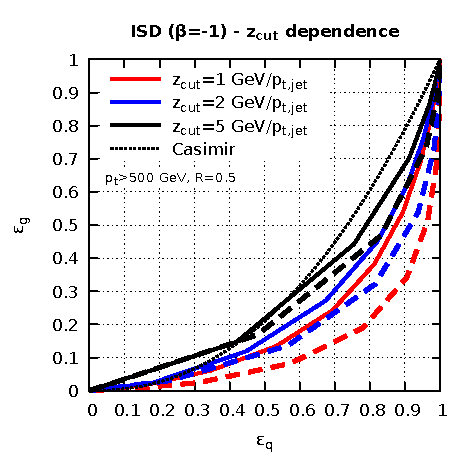
\includegraphics[width=0.48\textwidth,page=1]{figures/isd-roc.pdf}%
  \hfill%
  \includegraphics[width=0.48\textwidth,page=2]{figures/isd-roc.pdf}%
  \caption{Quark-gluon discrimination (ROC curve) using Iterated
    SoftDrop. The left plot uses a fixed jet $p_t$ cut and varies the
    Iterated \SD cut (defined as in
    Fig.~\ref{fig:isd-distrib-v-ktcut}. For the right plot, $\zcut$ is
    fixed to 2~GeV$/(p_tR)$ and the cut on the jet $p_t$ is
    varied.}\label{fig:isd-roc}
\end{figure}  

\paragraph{Quark-gluon discrimination.}
%
The ROC curves obtained for quark-gluon discrimination are presented
in Fig.~\ref{fig:isd-roc}, for Pythia (solid) and the LL analytic
calculations (dashed).
%
The left plot corresponds to the distributions shown in
Fig.~\ref{fig:isd-distrib-v-ktcut}.
%
First, we see that the discriminating power improves with lower
$\zcut$. This is expected since the phase-space for emissions
increases and so does $\nu$.
%
Then, although the analytic calculation tends to over-estimate the
discriminating power, the generic trend remains decently reproduced
and we see, in particular, that the agreement is better at larger
$\zcut$ where the distribution is expected to have smaller
non-perturbative corrections.
%
It is  worth pointing  out that  the flavour-changing  effects briefly
mentioned above  and appearing at  NLL accuracy would have  the effect
that  quark and  gluon jets  would  become more  similar as  we go  to
smaller angles, hence reducing the discriminating power.

Finally, the right plot of Fig.~\ref{fig:isd-roc} shows that the
discriminating power of ISD multiplicity improves at larger
$p_t$ (for a fixed $k_t$ cut).
%
This is again a consequence of the fact that the phase-space
available for emissions, and hence $\nu$, increases.
%
This contrasts with the angularities discussed
previously: while the latter remain close to Casimir scaling at any
energy, the performance of ISD multiplicity improves for
larger jet $p_t$.


\section{Performance and robustness}\label{sec:qg-perf-robustness}

To conclude this study of quark-gluon tagging, we compare several
quark-gluon discriminators in terms of both their performance and
their robustness.
%
This is based on Pythia8 Monte Carlo simulations and we reiterate the
caveat that the quark-gluon separation varies between Monte Carlo
(cf.~\cite{Badger:2016bpw}), so this should be taken as a highlight of
the main features rather than a full study.
%
The main goal of this discussion is to stress more explicitly that, as
introduced in Sec.~\ref{sec:performance-intro}, a high-quality
substructure tool needs obviously to have a strong discriminating
power, but at the same time it small sensitivity to non-perturbative effects is
also desirable.

We first specify our quality measures for performance and
robustness.
%
For this, let us consider a given quark-gluon discriminator at a fixed
working point (\ie a given cut value). To treat quarks and gluons
symmetrically, we define performance as the geometric mean of the quark
significance and the gluon significance:
\begin{equation}
\Gamma_\text{sym} = \sqrt{\frac{\epsilon_q}{\sqrt{\epsilon_g}}\frac{1-\epsilon_g}{\sqrt{1-\epsilon_q}}},
\end{equation}
where one has used the fact that to tag gluon jets, one would impose a
cut $v>v_\text{cut}$ and $\epsilon_{v>v_\text{cut}}=1-\epsilon_{v<v_\text{cut}}$.
%
Robustness is then quantified through resilience, as introduced in
Sec.~\ref{sec:performance-intro}, Eq.~(\ref{eq:resilience}). For
simplicity, we will focus here on the resilience against
non-perturbative effects including both hadronisation and the
Underlying Event (UE). These effects could be studied separately but this
goes beyond the scope of this book. We note however that in our case,
resilience is dominated by hadronisation effects, with UE having a much smaller impact.
%
Finally, note that both the performance $\Gamma_\text{sym}$ and the
resilience $\zeta$ can be computed for any fixed cut on a shape or
multiplicity.

\begin{figure}[t]
  \includegraphics[width=0.48\textwidth,page=3]{figures/qg-rocs.pdf}%
  \hfill%
  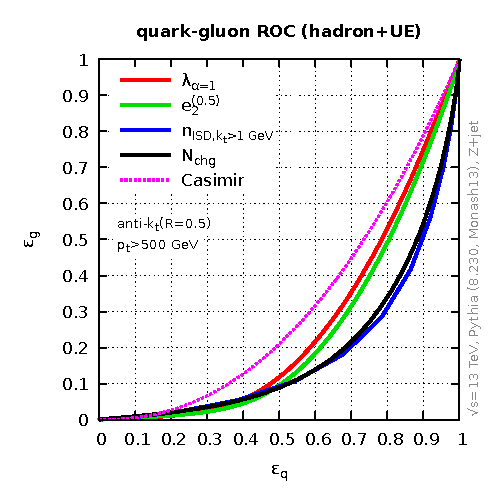
\includegraphics[width=0.48\textwidth,page=1]{figures/qg-rocs.pdf}
  \caption{ROC curves for a representative series of quark-gluon
    taggers: broadening, $\lambda_{\alpha=1}$ (red),
    energy-correlation function $e_2^{(\alpha=0.5)}$ (green), Iterated
    \SD with $\beta=-1$ and $\zcut=1~\text{GeV}/p_{t,\text{jet}}$, and the
    charged track multiplicity. All the results are shown for Pythia8
    simulations with a jet $p_t$ cut of 500~GeV. The left plot
    corresponds to parton-level events while the right plot
    corresponds to full simulations including hadronisation and the
    Underlying Event. The charged-track multiplicity is not shown at 
    parton level.}\label{fig:qg-roc-summary}
\end{figure}

First, we compare the performance of a few representative tools
discussed earlier in this section: girth or broadening, equivalent to
the angularity $\lambda_{\alpha=1}$, energy-correlation function
$e_2^{(\alpha=0.5)}$, the ISD multiplicity with
$\zcut=1~\text{GeV}/p_{t,jet}$ (corresponding to a $k_t$ cut of
1~GeV), and the charged track multiplicity.
%
The ROC curves are shown on Fig.~\ref{fig:qg-roc-summary} for Pythia8
simulations at parton level (left) and at hadron level including the
Underlying Event (right).
%
At small quark efficiency ($\epsilon_q\lesssim 0.5$) angularities and
energy correlation functions tend to give a better discriminating
power. At larger quark efficiency multiplicity-based discriminators show a better performance, with the
ISD and charged-track multiplicities behaving similarly.

\begin{figure}[t!]
  \centerline{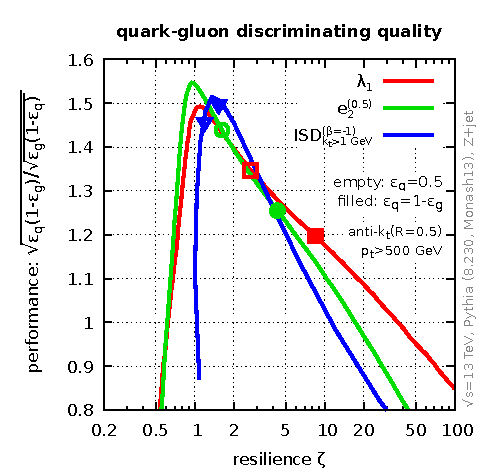
\includegraphics[width=0.48\textwidth,page=1]{figures/qg-performance.pdf}}
  \caption{Quark-gluon tagging quality: performance v.\ resilience for
    the taggers used in Fig.~\ref{fig:qg-roc-summary}. The curves
    correspond to varying the cut on the jet shape or
    multiplicity. Solid (empty) points correspond to the specific
    working point for which $\epsilon_q=1-\epsilon_g$
    ($\epsilon_q=0.5$). Performance is computed at hadron+UE level and
    resilience includes both hadronisation and UE
    effects.}\label{fig:qg-quality}
\end{figure}

We now discuss both the performance and resilience of our
representative sample of quark-gluon taggers. This is first shown on
Fig.~\ref{fig:qg-quality} for the full ROC curves corresponding to
Fig.~\ref{fig:qg-roc-summary}, \ie where the lines are obtained by
varying the cut on the shape or multiplicity. The empty symbols
correspond to a fixed quark efficiency of 0.5 at hadron+UE level,
while the solid symbols correspond to a symmetric working point where
$\epsilon_q=1-\epsilon_g$ (at hadron+UE level).\footnote{For
  multiplicity-based observables, we have interpolated linearly
  between the discrete multiplicities.} The charged-track
multiplicity is not plotted simply because it is not well-defined at
parton level.

We see that angularities and ECFs give their best performance at
relatively low quark efficiency, corresponding to a fairly low
resilience. As the quark efficiency decreases (going to
$\epsilon_q=0.5$, then $\epsilon_q=1-\epsilon_g$) performance
decreases but one gains resilience. A similar behaviour is seen for
ISD although the highest performance is observed for larger quark
efficiencies and large resilience at yet larger quark efficiencies.
%
For our 500-GeV sample, the best performance is achieved by
ECF($\alpha=0.5$) closely followed by ISD, with the latter showing a
slightly better resilience against non-perturbative effects.
%
At lower $\Gamma_\text{sym}$ this is inverted, with shape-based
variables becoming more resilient than ISD. 

The crucial observation one draws from Fig.~\ref{fig:qg-quality} is
that, generally speaking, there is a trade-off between performance and
resilience.
%
This pattern is seen repeatedly in substructure studies (we will see
another example in our two-prong-tagger study in the next chapter) and can be
understood in the following way: tagging constrains patterns of
radiation inside a jet; usually, increasing the phase-space over which
we include the radiation, and in particular the region of soft
emissions, means increasing the information one includes in the tagger
and hence increasing the performance; at the same time, the region of soft
emissions being the one which is most sensitive to hadronisation and
the Underlying Event, one also reduces resilience.

\begin{figure}[t!]
  \includegraphics[width=0.48\textwidth,page=3]{figures/qg-performance.pdf}%
  \hfill%
  \includegraphics[width=0.48\textwidth,page=2]{figures/qg-performance.pdf}
  \caption{Plot of performance v.\ resilience for quark-gluon taggers,
    as in Fig.~\ref{fig:qg-quality}, varying the cut on the jet $p_t$,
    using the working point $\epsilon_q=1-\epsilon_g$. The left plot
    shows two different choices of parameters for the taggers. The
    right plot shows two different levels of
    grooming. }\label{fig:qg-quality-ptdep}
\end{figure}


\begin{figure}[t!]
  \includegraphics[width=0.48\textwidth,page=7]{figures/qg-performance.pdf}%
  \hfill%
  \includegraphics[width=0.48\textwidth,page=6]{figures/qg-performance.pdf}%
  \caption{Plot of performance v.\ resilience for quark-gluon taggers,
    as in Fig.~\ref{fig:qg-quality-ptdep} but now using the working
    point that maximises performance for each
    setup.}\label{fig:qg-quality-ptdep-best-perf}
\end{figure}

To finish this study of quark-gluon taggers, we show in
Fig.~\ref{fig:qg-quality-ptdep} how the quark-gluon tagging quality
varies with the jet $p_t$. From small to big symbols, we have used
$p_t>500$~GeV, $p_t>1$~TeV and $p_t>2$~TeV, and we have focused on the
point for which $\epsilon_q=1-\epsilon_g$.
%
The left plot shows this for two different choices of parameters (two
exponents for angularities and ECFs and two $\zcut$ for ISD).
%
We see clearly that, as expected from our earlier studies, the
performance of ISD increases with the jet $p_t$ while that of
shape-based taggers remains roughly constant. Conversely, shape-based
taggers become more resilient at larger $p_t$, highlighting again a
trade-off between performance and resilience.

The right plot of Fig.~\ref{fig:qg-quality-ptdep} shows two different
levels of grooming: the plain jet and a jet groomed with
mMDT\footnote{In the case of ISD, we have applied mMDT recursively,
  giving a behaviour equivalent to using $\beta=0$ and a $k_t$ cut as
  shown in the middle plot of Fig.~\ref{fig:lund-isd-lund}.}
%
The dependence on the jet $p_t$ is the same as what was already
observed for the left plot (although, for mMDT jets, the performance
of ISD only increases marginally). What is more interesting is that
one clearly sees that grooming has the effect of reducing the
performance and increasing the resilience.
%
Since grooming is (almost by definition) removing soft emissions at
large angles, this is another textbook example of a trade-off between
performance and resilience.
%
We note however that these conclusions are relatively sensitive to the
choice of working point. For example,
Fig.~\ref{fig:qg-quality-ptdep-best-perf} shows the same result as
Fig.~\ref{fig:qg-quality-ptdep} but now selecting for each method the
working point which maximises performance. In this case, we see that
all methods give similar results both in terms of performance and in
terms of resilience, with even a small preference for ECFs (with
$\alpha=0.5$) if one is looking for sheer performance. It is worth
pointing out that in this case the quark and gluon efficiencies are
relatively low, meaning that (i) one might be affected by issues
related to lower statistics and (ii) we are in a region where the
discreteness of ISD can have large effects which one would need to
address in a more complete study.\footnote{For the results of
  Fig.~\ref{fig:qg-quality-ptdep-best-perf} we have simply
  interpolated between different points in the distribution.}

As a final comment, we point out that, given the different
behaviours seen between shape-based taggers and multiplicity-based
taggers, it would be interesting to study their combination in a
multivariate analysis. It would also be interesting to see how recent
quark-gluon taggers based on deep learning techniques use the
information relevant for ECFs and ISD.



%% GS helper for auctex
%%% Local Variables:
%%% mode: latex
%%% TeX-master: "notes"
%%% End:

%  LocalWords:  supersymmetric Monash ECFs Casimir NLL WTA CMW Eq eq
%  LocalWords:  Eqs NLOJet MCFM ECF ISD dimensionful UE
